\chapter{System Development and Implementation}

This chapter describes the implementation of the CyberCase Intelligence Framework. Chapter 3 defined the system requirements, workflow, and design boundaries; this chapter shows how those decisions are implemented in the current Web Application, Backend API, database, document-ingestion services, analysis pipeline, and conditional MITRE service. The implementation is described from the current working code so that the behavior in this chapter can be traced to a concrete module or API boundary.

The term case source is used consistently in this chapter. A case source is the text that the case is allowed to use as an input, including a user-written narrative and text extracted from an uploaded document. A follow-up answer remains a conversation message and is carried as follow-up history during analysis; it is not silently promoted to a new source revision. MITRE ATT\&CK descriptions and retrieval results are external technical context, not facts about the case.

\section{Development Environment and Implementation Structure}

CyberCase is implemented as a case-owned Web Application supported by a Backend API and a separate technical retrieval service. The frontend is responsible for user interaction and cached server state. The backend owns authentication, case access, source admission, routing, deterministic policy, validation, and persistence. The RAG service is called through an HTTP client and is limited to external MITRE ATT\&CK context.

The Backend API uses a request-scoped execution model. A case analysis is performed inside the request that asked for it; there is no run table, queue, polling route, or background result-claiming protocol. The application startup check also refuses a multi-worker configuration because the current analysis contract is deliberately one request and one result path.

The source tree is divided by responsibility rather than by screen name. Routers translate HTTP requests into service calls, schemas define the API contract, models describe PostgreSQL persistence, services implement domain behavior, and the frontend consumes typed responses. This structure keeps the UI from deciding whether an analysis is current, whether a gap may be asked, or whether external context is evidence.

\begin{longtable}{@{}>{\raggedright\arraybackslash}p{0.20\textwidth} >{\raggedright\arraybackslash}p{0.30\textwidth} >{\raggedright\arraybackslash}p{0.46\textwidth}@{}}
\caption{Development environment and service technology}\label{tab:4-1}\\
\toprule
\textbf{Layer} & \textbf{Implementation} & \textbf{Main responsibility} \\
\midrule
\endfirsthead
\textbf{Layer} & \textbf{Implementation} & \textbf{Main responsibility} \\
\midrule
\endhead
Web Application & Next.js 16, React 19, TypeScript, Tailwind CSS 4, TanStack Query & Case library, case workspace, source intake, analysis display, chat, and report controls \\
Backend API & FastAPI, Pydantic, SQLAlchemy async, PostgreSQL, Alembic & Authentication, case ownership, source storage, workflow orchestration, analysis, chat, and reports \\
Document processing & PDF/DOCX parsers, image rendering, Typhoon document recognition & Convert supported files into text with page-aware provenance and warnings \\
External technical service & FastAPI RAG service, LangGraph, Qdrant, Neo4j, BGE-M3 & Retrieve optional MITRE ATT\&CK context after the applicability gate \\
Runtime & Docker Compose and one Backend API worker & Run the services with PostgreSQL and preserve request-scoped analysis behavior \\
\bottomrule
\end{longtable}

\begin{longtable}{@{}>{\raggedright\arraybackslash}p{0.20\textwidth} >{\raggedright\arraybackslash}p{0.30\textwidth} >{\raggedright\arraybackslash}p{0.46\textwidth}@{}}
\caption{Implementation modules and boundaries}\label{tab:4-2}\\
\toprule
\textbf{Module} & \textbf{Representative path} & \textbf{Implementation boundary} \\
\midrule
\endfirsthead
\textbf{Module} & \textbf{Representative path} & \textbf{Implementation boundary} \\
\midrule
\endhead
Authentication & backend/app/services/auth/ & Owns sessions, password handling, and browser-request authorization. \\
Case and source services & backend/app/services/cases/ and sources/ & Owns case access, documents, extracted text, source provenance, and source revisions. \\
Document ingestion & backend/app/services/document\_ingestion/ & Detects formats, parses native text, renders pages, and calls document recognition when required. \\
Analysis workflow & backend/app/services/workflow/ and analysis/ & Reads a source bundle, runs assessment and analysis steps, and stores only the result allowed by the source revision check. \\
Technical context & backend/app/services/analysis/mitre\_gate/ and steps/technical\_context.py & Decides whether MITRE context applies and isolates retrieval output from case facts. \\
Reports & backend/app/services/reports/ & Projects a stored validated analysis into a deterministic report and renders HTML or PDF. \\
Frontend data access & frontend/src/hooks/ and frontend/src/lib/api/ & Keeps server state in query caches and exposes typed API contracts to the workspace views. \\
\bottomrule
\end{longtable}

\begin{figure}[H]
\centering
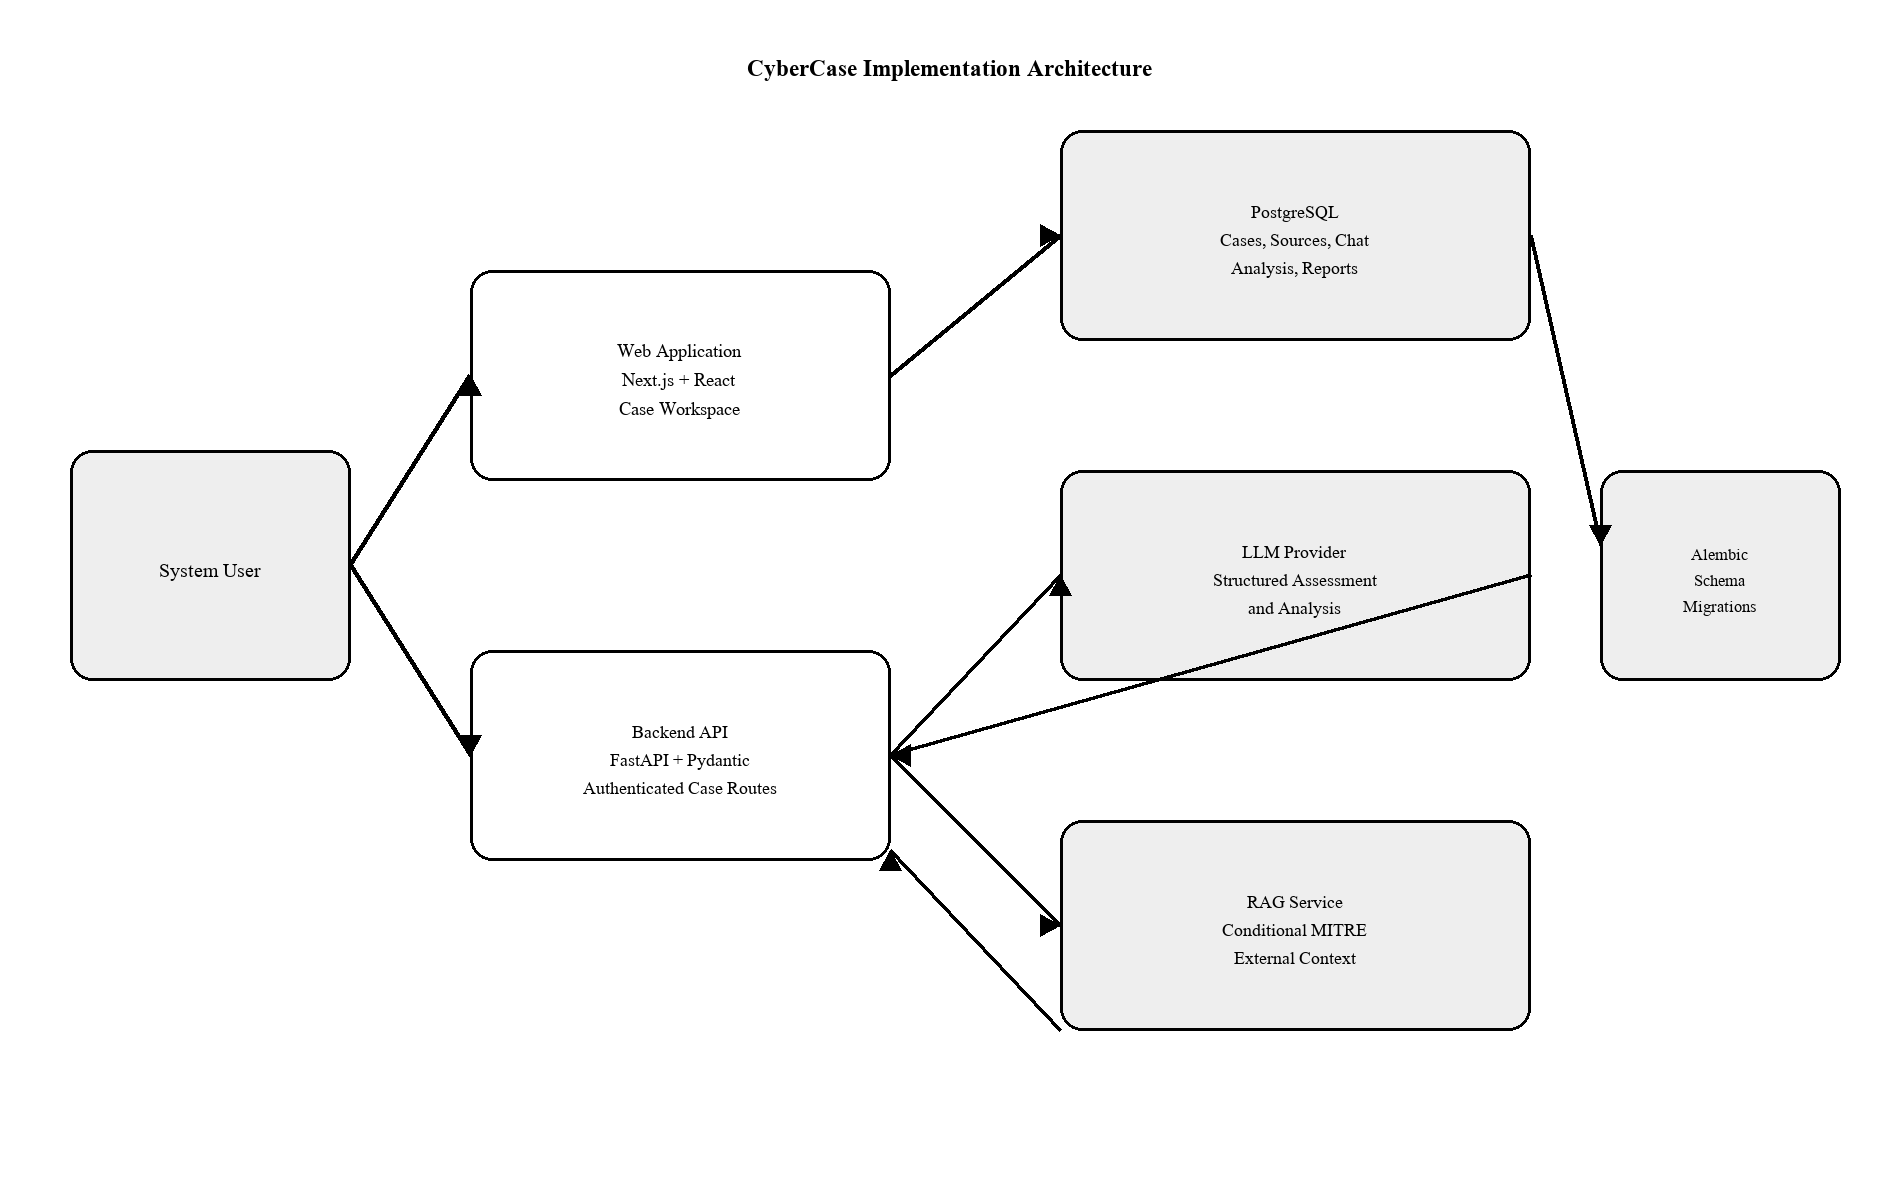
\includegraphics[width=0.96\textwidth]{figures/chapter4/figure-4-1.png}
\caption{CyberCase implementation architecture}\label{fig:4-1}
\end{figure}

\section{Case Material Preparation}

A case can receive a narrative directly from the user or a supported document. The intake route first validates the uploaded content and detects its document kind. A document is kept as the original case document, while the readable text is stored as a document extraction and then admitted as a case source. This separation allows the original file, extraction record, and text used by analysis to remain related without treating a parser output as a new type of case fact.

PDF processing is page-aware. Pages with usable native text use that text directly. When native text is missing or unusable, the page is rendered to an image and sent to the configured document-recognition provider. DOCX input is read from paragraphs and tables, and PNG or JPEG input is normalized as a single rendered page. The resulting page objects retain page number, extraction method, verification status, and warnings.

The stored provenance is later used when a quotation from a document is resolved to a page. The system therefore does not ask the language model to invent a page number. The model returns a source identifier and quotation; the binding step finds that quotation in the stored text and derives the document locator when page spans are available.

Every source mutation increments the case source\_revision. A source bundle carries the revision that it was read from. When analysis finishes, the storage transaction locks the case and refuses to save the result if the revision has changed during model processing. This prevents a result computed from an older input set from being presented as the current analysis.

\begin{longtable}{@{}>{\raggedright\arraybackslash}p{0.20\textwidth} >{\raggedright\arraybackslash}p{0.30\textwidth} >{\raggedright\arraybackslash}p{0.46\textwidth}@{}}
\caption{Supported source-intake paths}\label{tab:4-3}\\
\toprule
\textbf{Input} & \textbf{Processing path} & \textbf{Stored result} \\
\midrule
\endfirsthead
\textbf{Input} & \textbf{Processing path} & \textbf{Stored result} \\
\midrule
\endhead
Narrative text & Validate non-empty text and create a text case source & Exact text, source kind, metadata, and incremented source revision \\
Text-based PDF & Inspect pages and retain usable native text & Original document, extraction record, page text, provenance, and warnings \\
Scanned or low-text PDF & Render each unusable page and send it to document recognition & Page-level recognized text with machine-read or needs-review status \\
DOCX & Read paragraphs and tables through the document parser & Extracted text and document provenance \\
PNG or JPEG & Normalize the image and send one rendered page to document recognition & One-page extracted text and recognition provenance \\
\bottomrule
\end{longtable}

\begin{figure}[H]
\centering
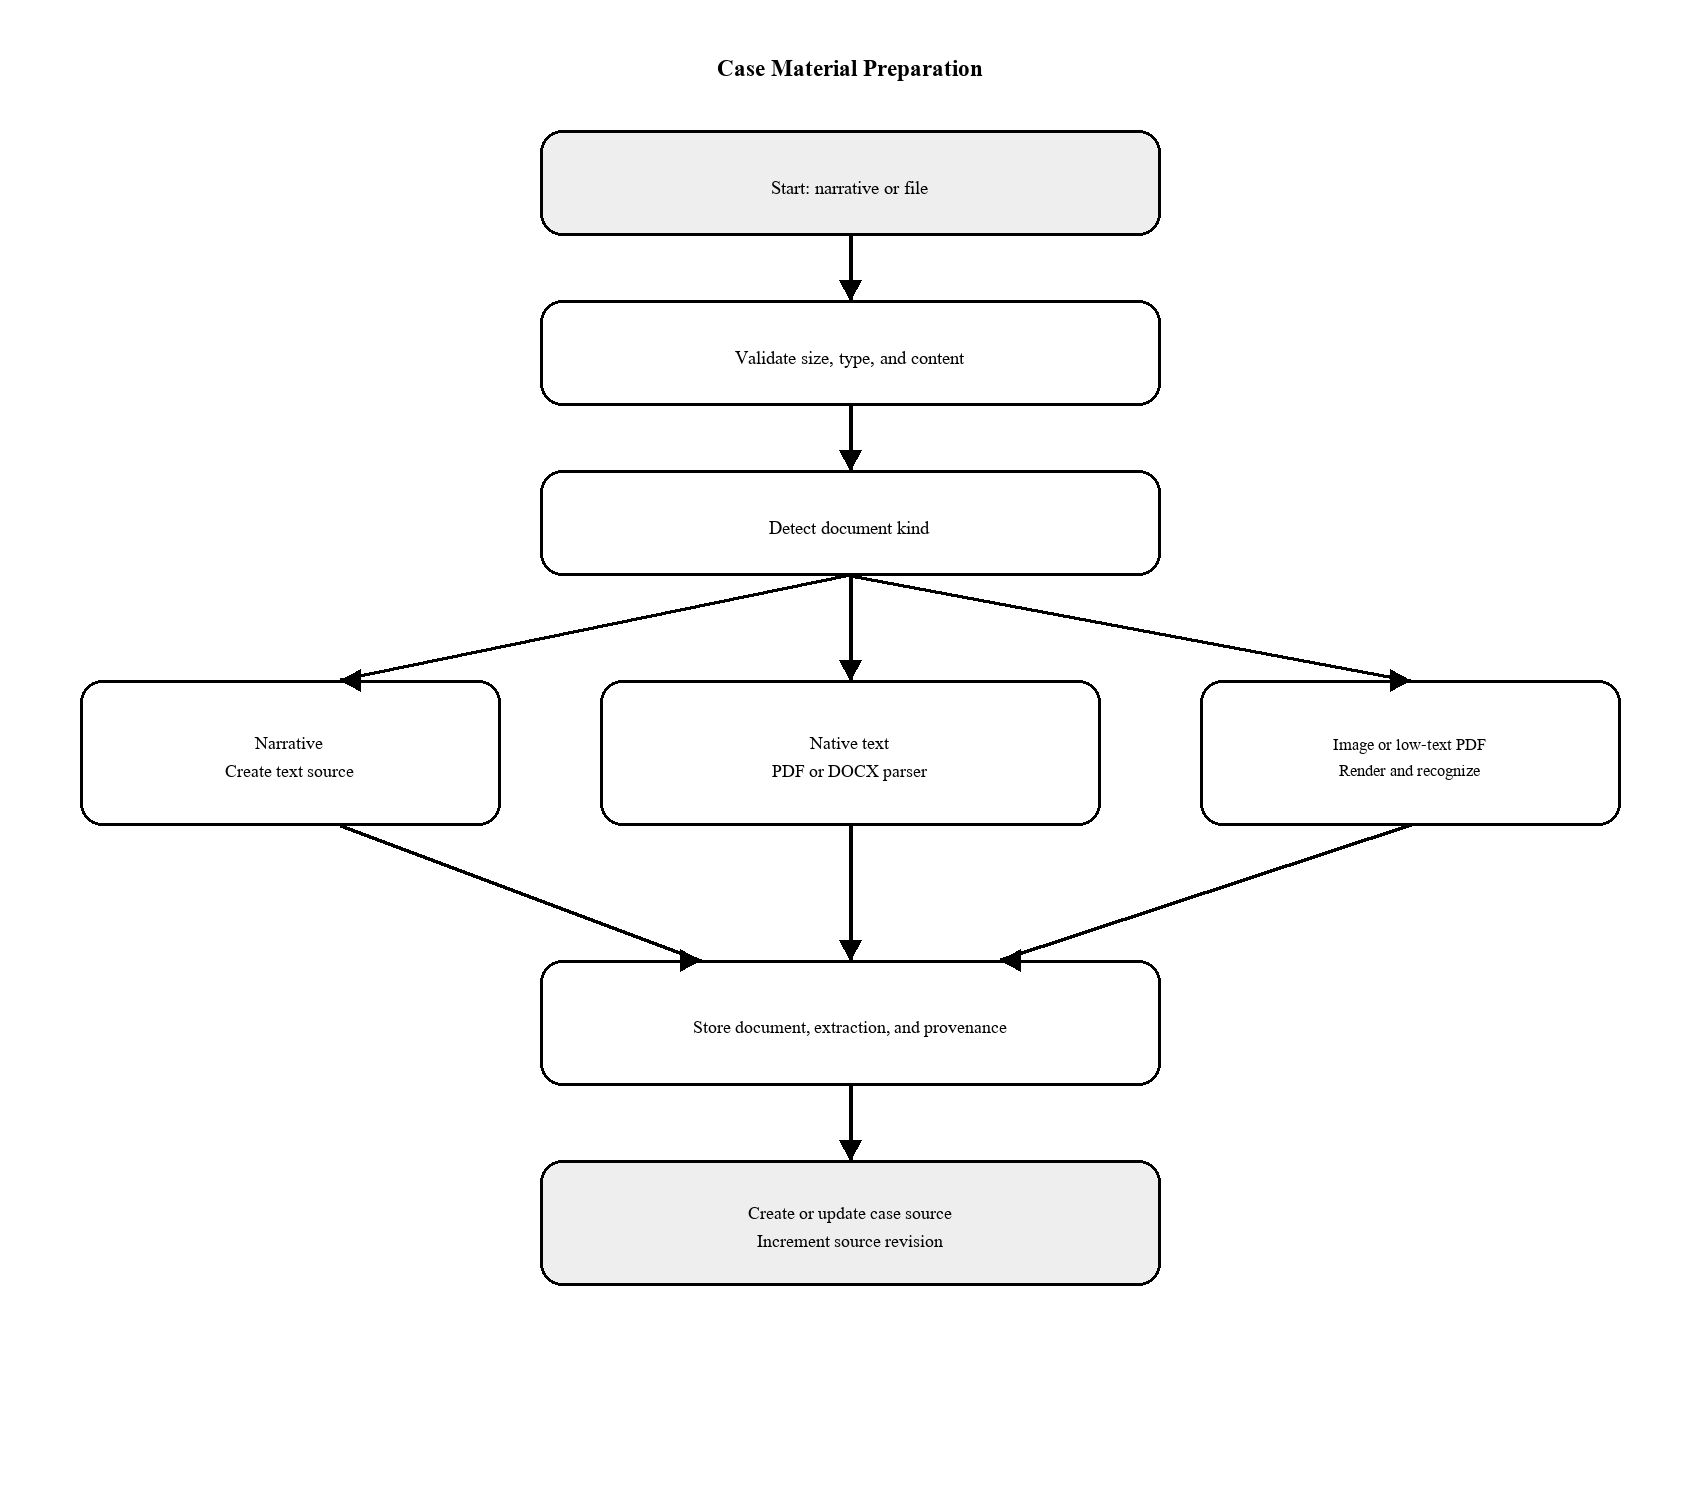
\includegraphics[width=0.96\textwidth]{figures/chapter4/figure-4-2.png}
\caption{Document and narrative intake flow}\label{fig:4-2}
\end{figure}

\section{Main Case Analysis}

The production analysis begins in the workflow service by reading the owned Case, active case sources, follow-up history, and reusable technical context. The database transaction ends before provider calls begin. The pipeline receives an immutable AnalysisInput, so its steps do not open a database connection or reach into persistence while semantic processing is in progress.

The first operation is gap assessment. The assessment uses a strict gaps-only contract and is not the final case analysis. The deterministic decide\_followup function then filters the returned gaps by priority, askability, clarification-question presence, previously asked keys, round budget, and per-round budget. If an eligible gap remains, the request stores an assessment result and a follow-up question and stops before technical retrieval and the main analysis call.

If the decision is Proceed, the pipeline runs conditional technical augmentation, writes one structured CaseAnalysisTrace, and binds that trace back to the case. The binding step does not replace the model's analysis with a second semantic analysis. It validates the identifiers and quotations, trims references that do not belong to the case, records the resulting grounding counts, and returns a result that can be stored as validated.

The final storage transaction checks source\_revision again. A validated result records the source revision, schema version, structured trace, pipeline configuration, technical augmentation metadata, and optional reusable retrieval context. The Case points to the latest validated result, while an assessment row remains a record of the follow-up decision and does not become the latest complete analysis.

\begin{longtable}{@{}>{\raggedright\arraybackslash}p{0.15\textwidth} >{\raggedright\arraybackslash}p{0.19\textwidth} >{\raggedright\arraybackslash}p{0.46\textwidth} >{\raggedright\arraybackslash}p{0.14\textwidth}@{}}
\caption{Production analysis steps}\label{tab:4-4}\\
\toprule
\textbf{Order} & \textbf{Step} & \textbf{Purpose} & \textbf{Output} \\
\midrule
\endfirsthead
\textbf{Order} & \textbf{Step} & \textbf{Purpose} & \textbf{Output} \\
\midrule
\endhead
1 & Assess gaps & Ask the model for a strict gaps-only assessment using the source bundle and follow-up history. & CaseAssessmentTrace \\
2 & Decide follow-up & Apply deterministic priority, askability, duplicate, round, and per-round limits. & Ask or Proceed \\
3 & Retrieve technical context & Run the MITRE gate and call or reuse RAG context only when applicable. & Augmentation status and optional MITRE table \\
4 & Write analysis & Make one structured analysis call using the admitted sources and permitted context. & CaseAnalysisTrace \\
5 & Bind to case & Resolve source identifiers, exact quotations, page locators, and MITRE associations. & Validated trace and grounding report \\
\bottomrule
\end{longtable}

\begin{figure}[H]
\centering
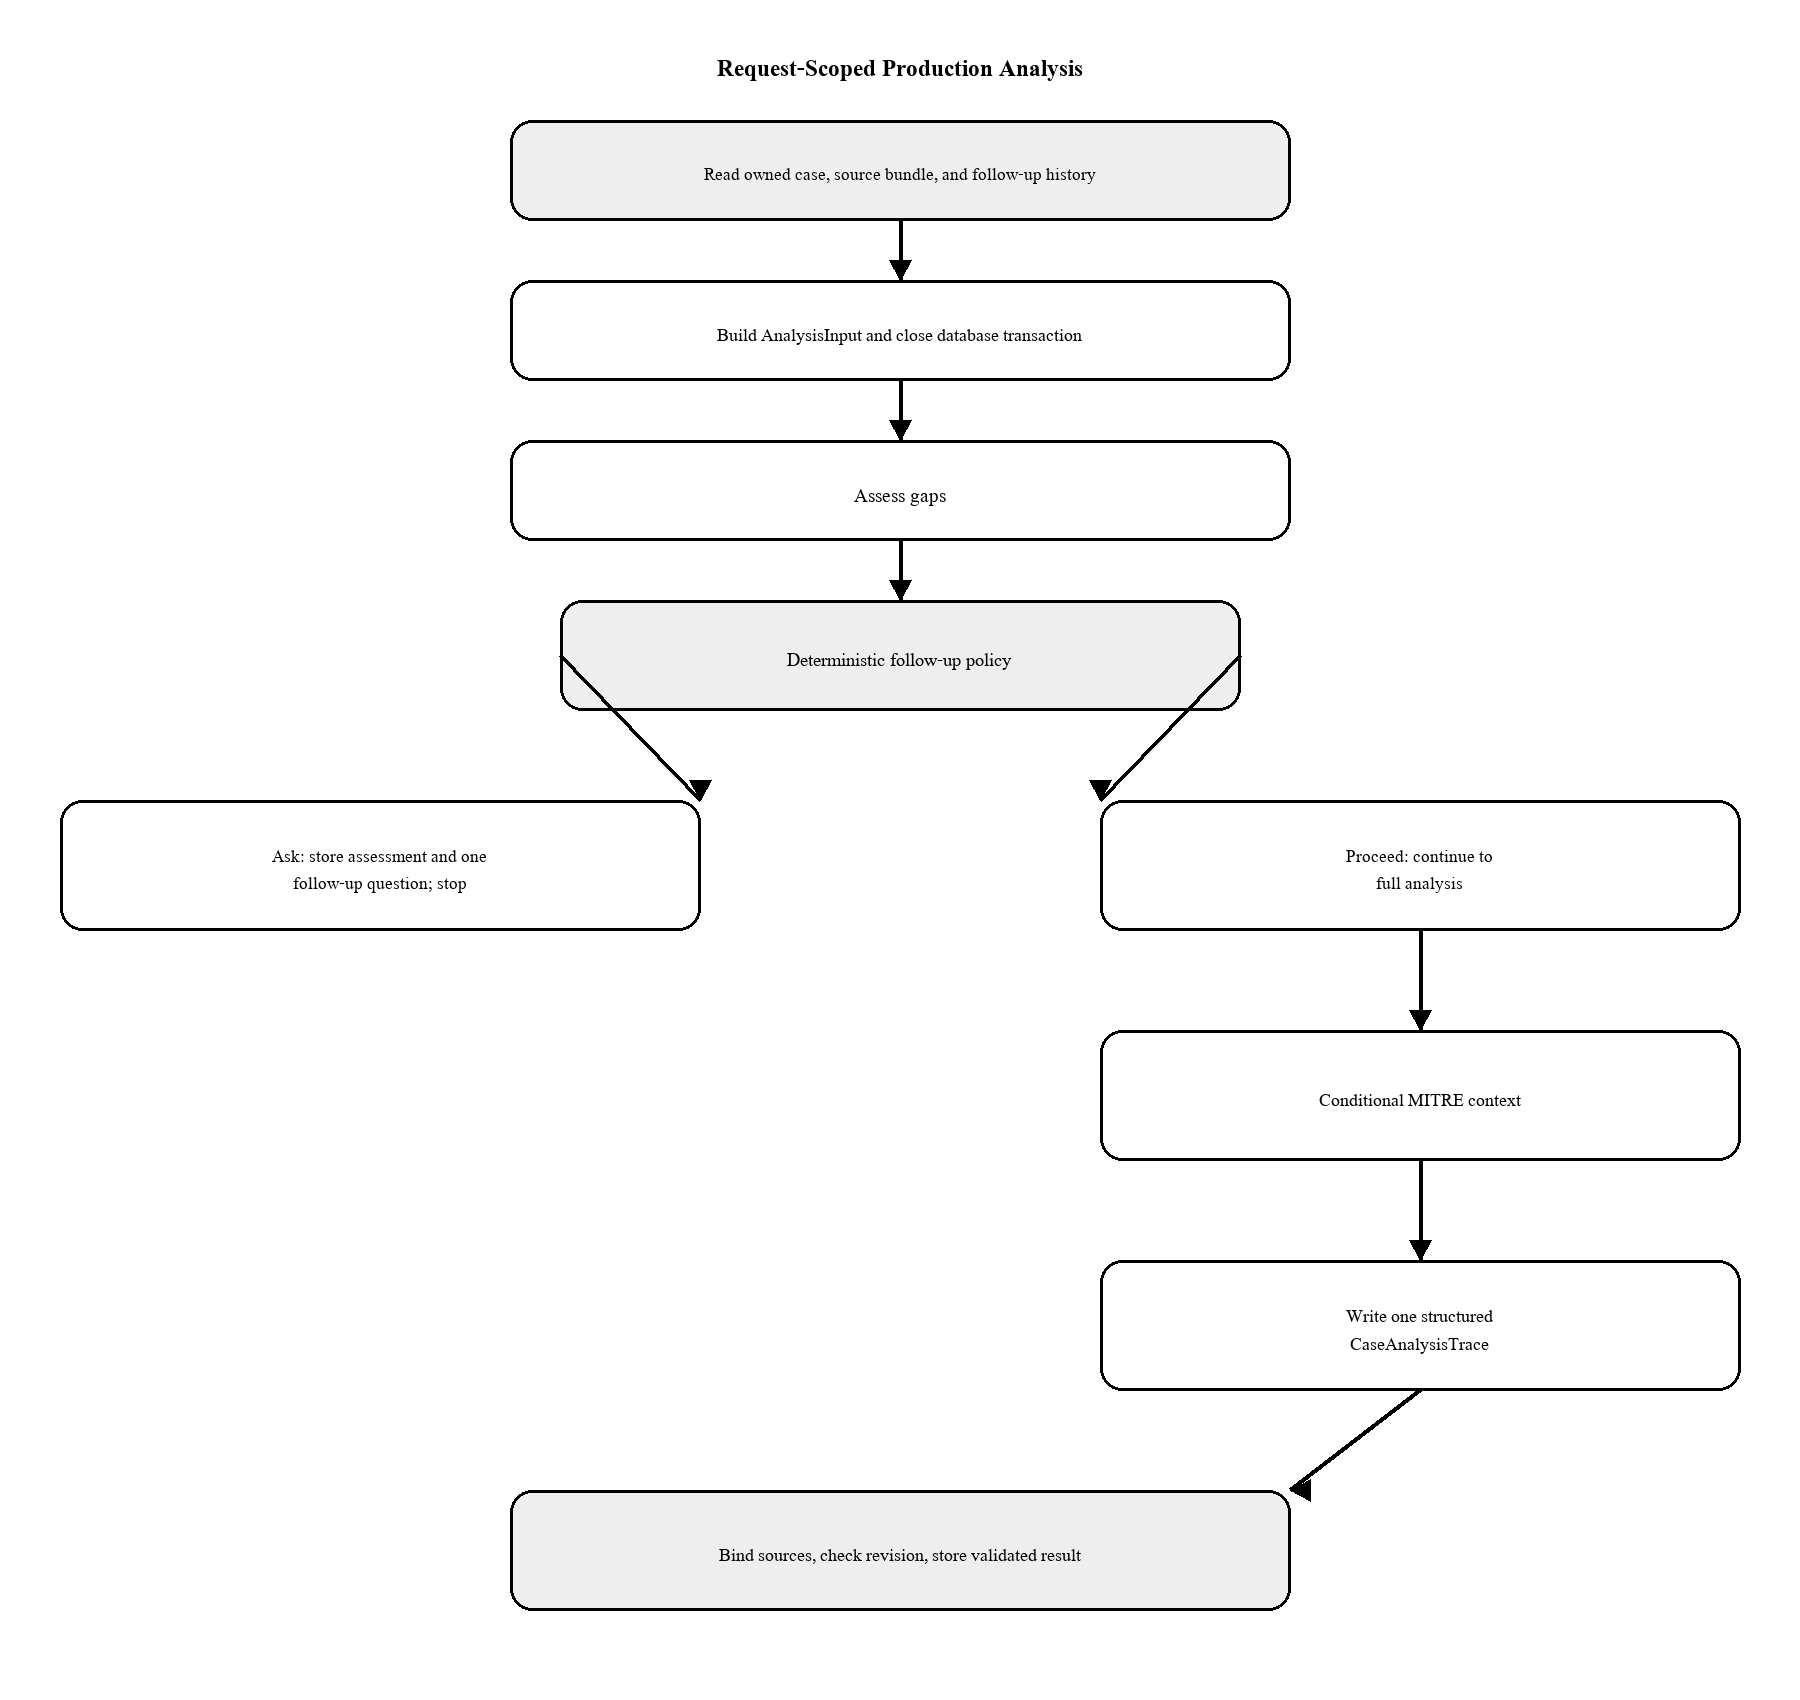
\includegraphics[width=0.96\textwidth]{figures/chapter4/figure-4-3.png}
\caption{Production case-analysis flow}\label{fig:4-3}
\end{figure}

\section{Conditional Technical Knowledge Retrieval}

MITRE ATT\&CK is implemented as an optional external-context stage rather than as the identity of the product. The configured gate reads the case sources and returns an applicability record. The current gate selector supports the normal language-model gate, an optional encoder gate, and a never-applicable mode used to measure the value of retrieval without changing the rest of the analysis pipeline.

When the gate returns SKIP, the pipeline continues to the general analysis without sending a retrieval request. When the gate allows retrieval, the Backend sends a bounded query to the RAG service and validates the returned retrieval\_context\_id, context text, and MITRE table. A failed request, invalid response, or insufficient context is recorded as a technical-augmentation status; it does not turn the general case analysis into an external knowledge answer.

The retrieved table is available to the analysis as technical context and is stored in external\_context\_json with its status and retrieval identifier. MITRE associations are retained only when they name a technique present in the retrieved table and point to known analysis claims. This makes the technical appendix traceable to the external retrieval response without allowing it to support a case claim.

A reusable context can be read from the most recent result when its context key matches the current source\_revision and the number of answered follow-up exchanges. The key prevents a previous retrieval from being silently reused after the case material or the answered follow-up history has changed.

\begin{figure}[H]
\centering
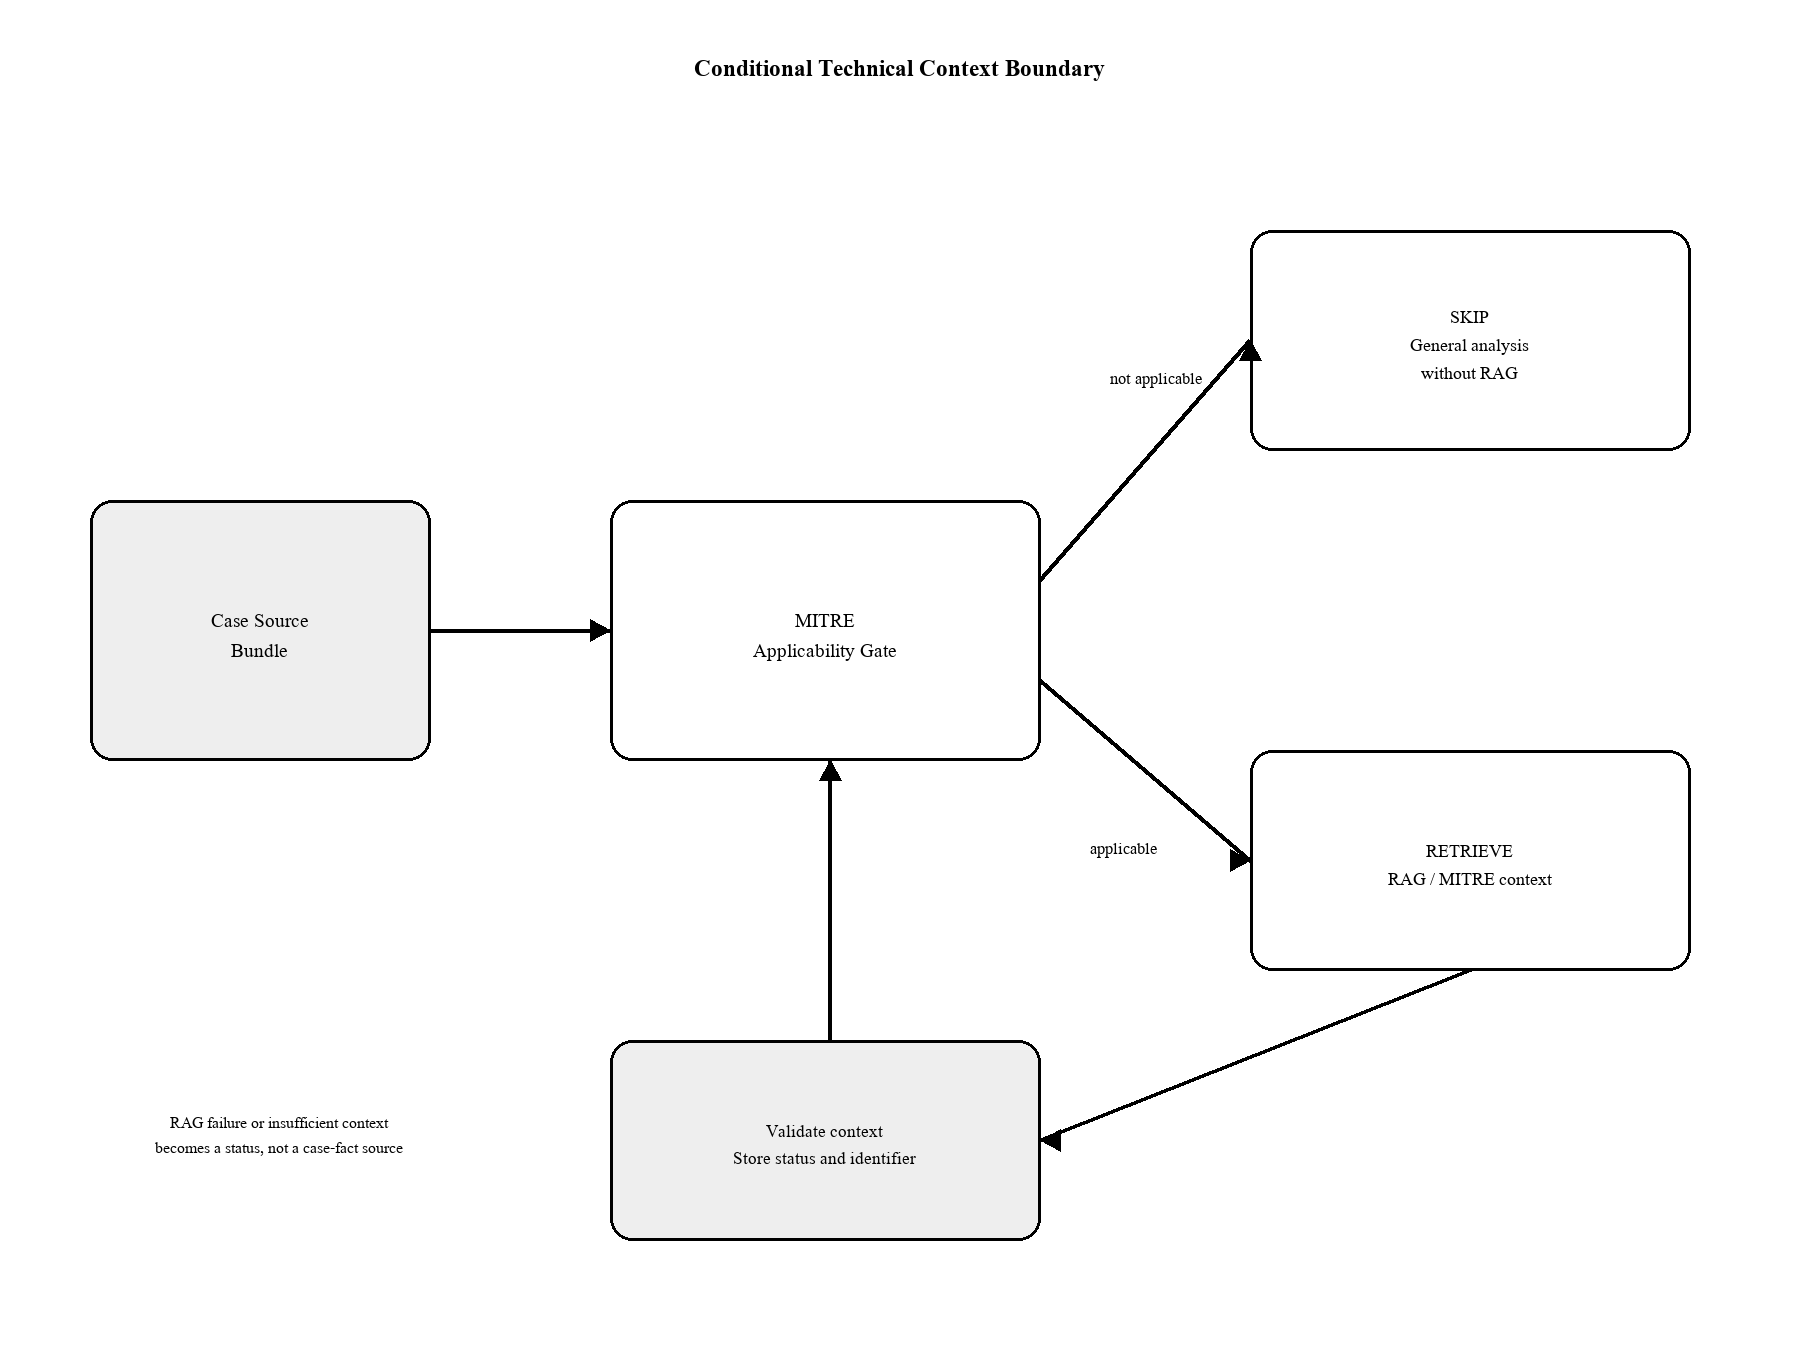
\includegraphics[width=0.96\textwidth]{figures/chapter4/figure-4-4.png}
\caption{Conditional MITRE context boundary}\label{fig:4-4}
\end{figure}

\section{Gap Analysis and Follow-up}

The analysis contract distinguishes unresolved information from ordinary findings. A gap identifies a topic, status, description, reason, affected claims, priority, askable flag, and optional clarification question. The statuses NOT\_PROVIDED, EXPLICITLY\_UNKNOWN, AMBIGUOUS, and CONFLICTING allow the result to preserve uncertainty instead of forcing every missing fact into a question.

The follow-up policy is deterministic and bounded. Only high-priority, askable gaps with a question and a gap key are candidates. A key already asked in the case is excluded. The policy returns either Ask with one selected gap or Proceed with a reason such as no eligible gap, gaps exhausted, maximum rounds reached, or the current round budget being spent.

The chat service keeps one unanswered follow-up question outstanding. A reply is stored as a follow-up answer message linked to the question. It remains part of the follow-up history read by the next analysis and does not increment source\_revision. For citation binding, an answered exchange is represented as a temporary source-like item with a stable QA identifier; this is an in-memory analysis representation, not an automatic persistence mutation.

When the round still has another selected question, the chat returns that question. When the round is complete, the service starts the next request-scoped analysis with the accumulated follow-up history. General chat questions follow a separate answer path and are not allowed to create incident claims or retrieve new external knowledge about the case.

\begin{longtable}{@{}>{\raggedright\arraybackslash}p{0.28\textwidth} >{\raggedright\arraybackslash}p{0.68\textwidth}@{}}
\caption{Gap states and follow-up policy}\label{tab:4-5}\\
\toprule
\textbf{Field or rule} & \textbf{Implementation meaning} \\
\midrule
\endfirsthead
\textbf{Field or rule} & \textbf{Implementation meaning} \\
\midrule
\endhead
Gap status & NOT\_PROVIDED, EXPLICITLY\_UNKNOWN, AMBIGUOUS, or CONFLICTING describes why information is unresolved. \\
Askable & The gap may be asked only when the validated gap remains askable and includes a clarification question. \\
Priority & Only high-priority gaps enter the normal follow-up candidate list. \\
One outstanding question & The answer is unambiguous because the chat holds at most one unanswered follow-up question. \\
Round limit & The case stops asking after the configured maximum number of rounds. \\
Per-round limit & A round can expose only the configured number of gaps before the case is analysed again. \\
\bottomrule
\end{longtable}

\begin{figure}[H]
\centering
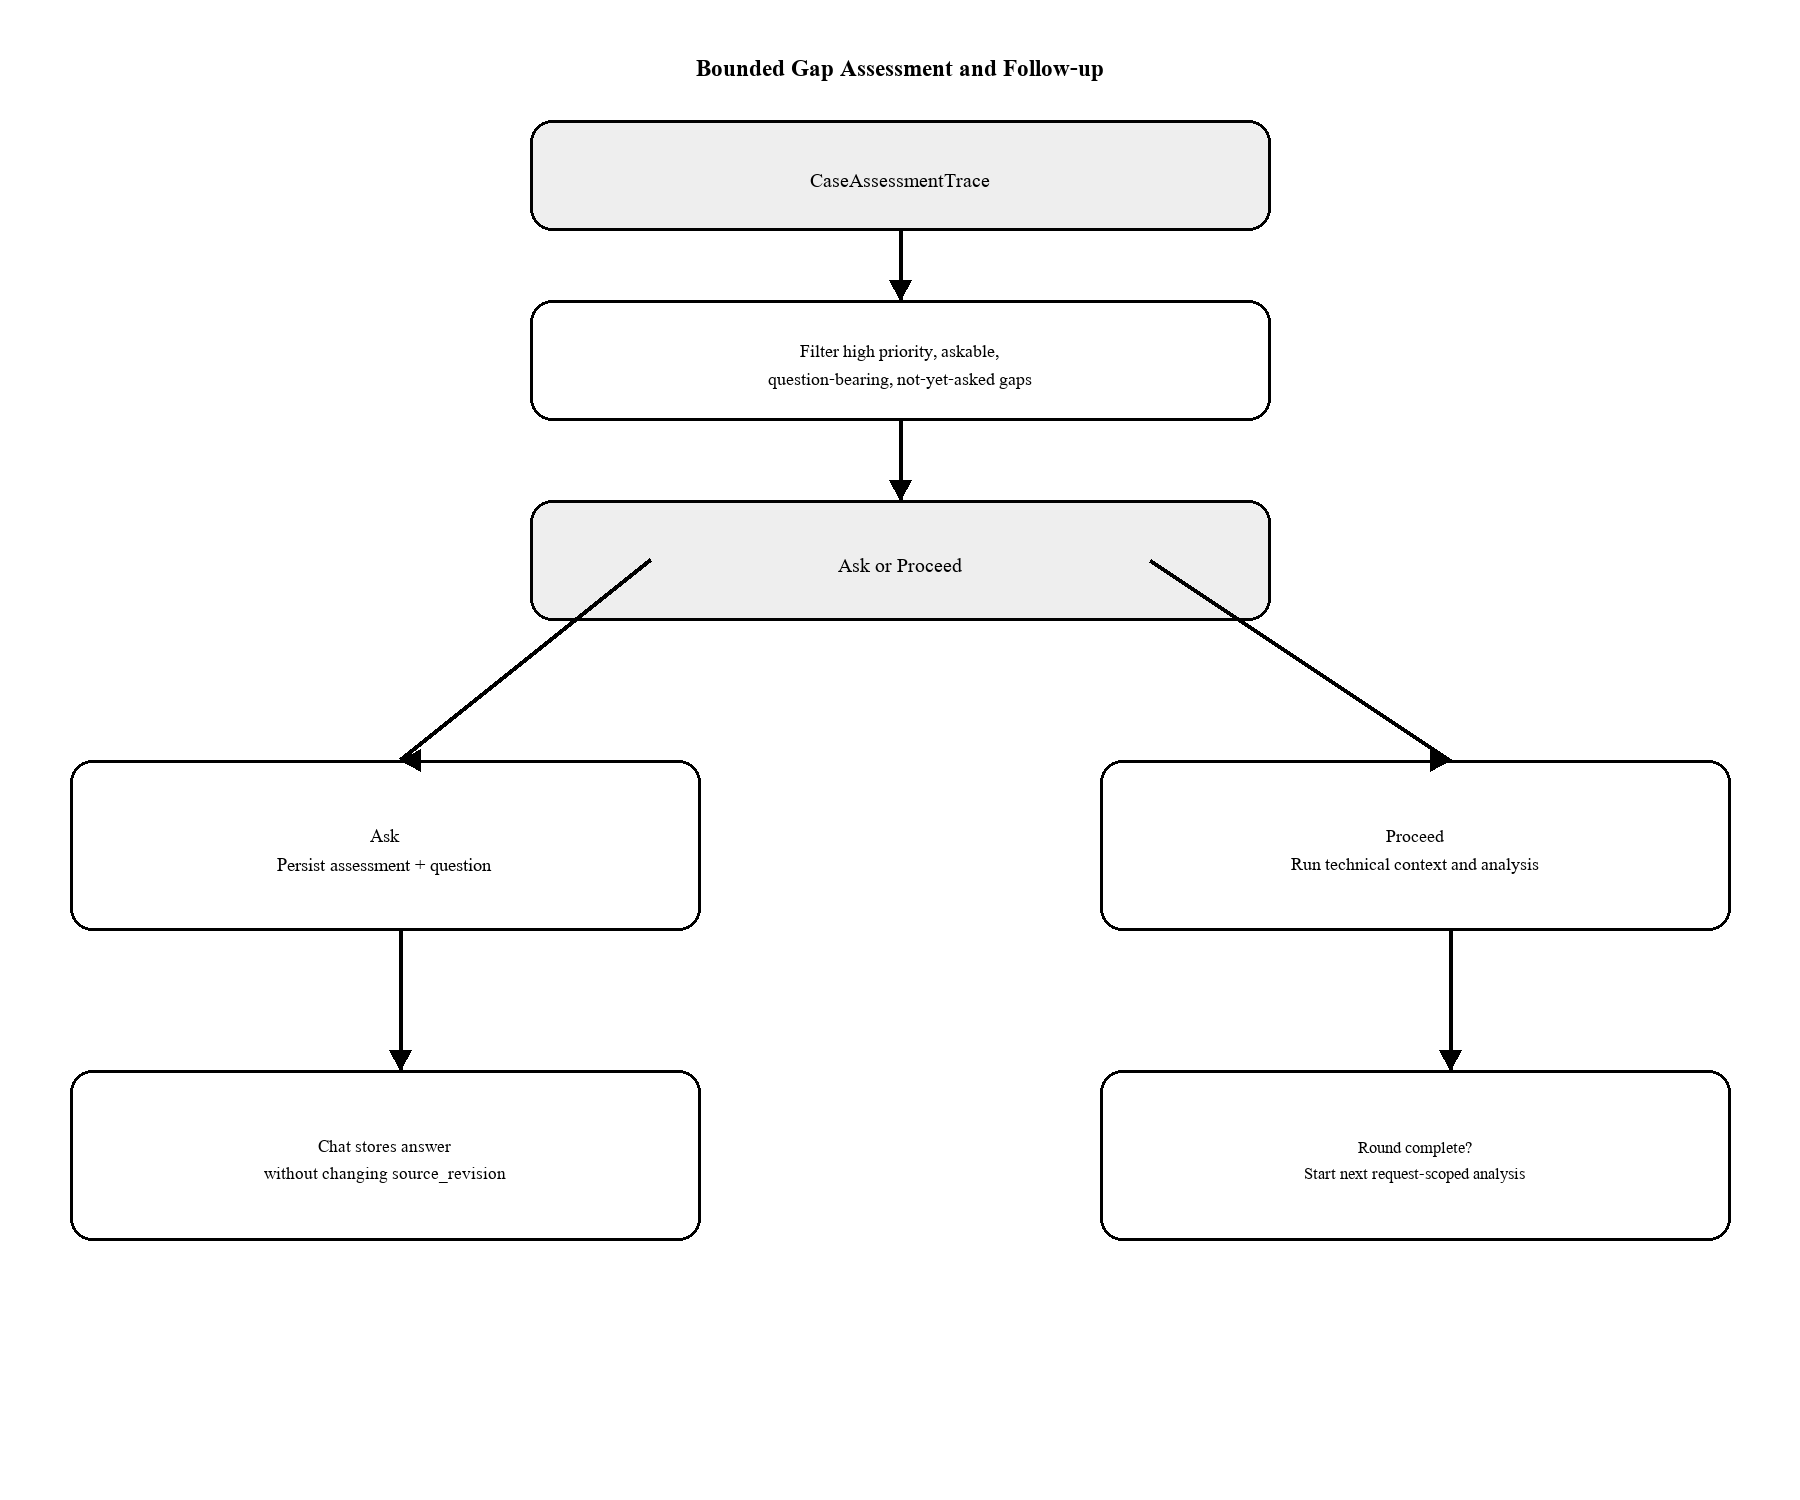
\includegraphics[width=0.96\textwidth]{figures/chapter4/figure-4-5.png}
\caption{Bounded gap assessment and follow-up}\label{fig:4-5}
\end{figure}

\section{Source Binding and Persistence}

The structured analysis is accepted only after local contract validation and source binding. Each claim may name supporting or contradicting source identifiers and exact quotations. The binding registry contains the active case sources, document provenance, and answered follow-up exchanges. A source identifier outside that registry is removed from the claim, while a quotation that cannot be found is omitted and counted in the grounding report.

The resolver can align minor quotation differences to the source text, resolve page numbers from stored page spans, remove duplicate claims by claim identifier, and keep only MITRE associations that refer to retrieved techniques and existing claim identifiers. Related parties, timeline entries, impacts, and gaps are trimmed so that they cannot point to a claim that was removed during binding.

The grounding report records claims, claimed citations, verified citations, paraphrased citations, unfound citations, claims without support, duplicated claims, associations outside the retrieved context, sources cited, and total sources. These counts preserve a measurable record of what survived validation without pretending that quotation existence proves semantic entailment.

PostgreSQL stores the Case aggregate and the records related to it. The database model uses foreign keys, check constraints, indexes, and Alembic migrations. Analysis results have two meaningful stored statuses: assessment for a gap-only stopping point and validated for a complete structured analysis. The report table binds one saved report to one analysis result and assigns a version number within the case.

\begin{longtable}{@{}>{\raggedright\arraybackslash}p{0.28\textwidth} >{\raggedright\arraybackslash}p{0.68\textwidth}@{}}
\caption{Core persistence objects}\label{tab:4-6}\\
\toprule
\textbf{Object} & \textbf{Stored implementation role} \\
\midrule
\endfirsthead
\textbf{Object} & \textbf{Stored implementation role} \\
\midrule
\endhead
users & Authenticated user identity and account ownership. \\
cases & Case aggregate, title, source\_revision, and latest validated analysis pointer. \\
case\_documents & Original uploaded file metadata and deferred binary content. \\
document\_extractions & Provider, configuration, extracted text, provenance, and warnings. \\
case\_sources & Exact text admitted to the case together with source kind and provenance. \\
chat\_messages & Conversation, follow-up questions, follow-up answers, and analysis publications. \\
case\_analysis\_results & Assessment or validated analysis, source revision, structured trace, and external-context metadata. \\
case\_reports & Versioned deterministic report bound to one analysis result. \\
\bottomrule
\end{longtable}

\begin{figure}[H]
\centering
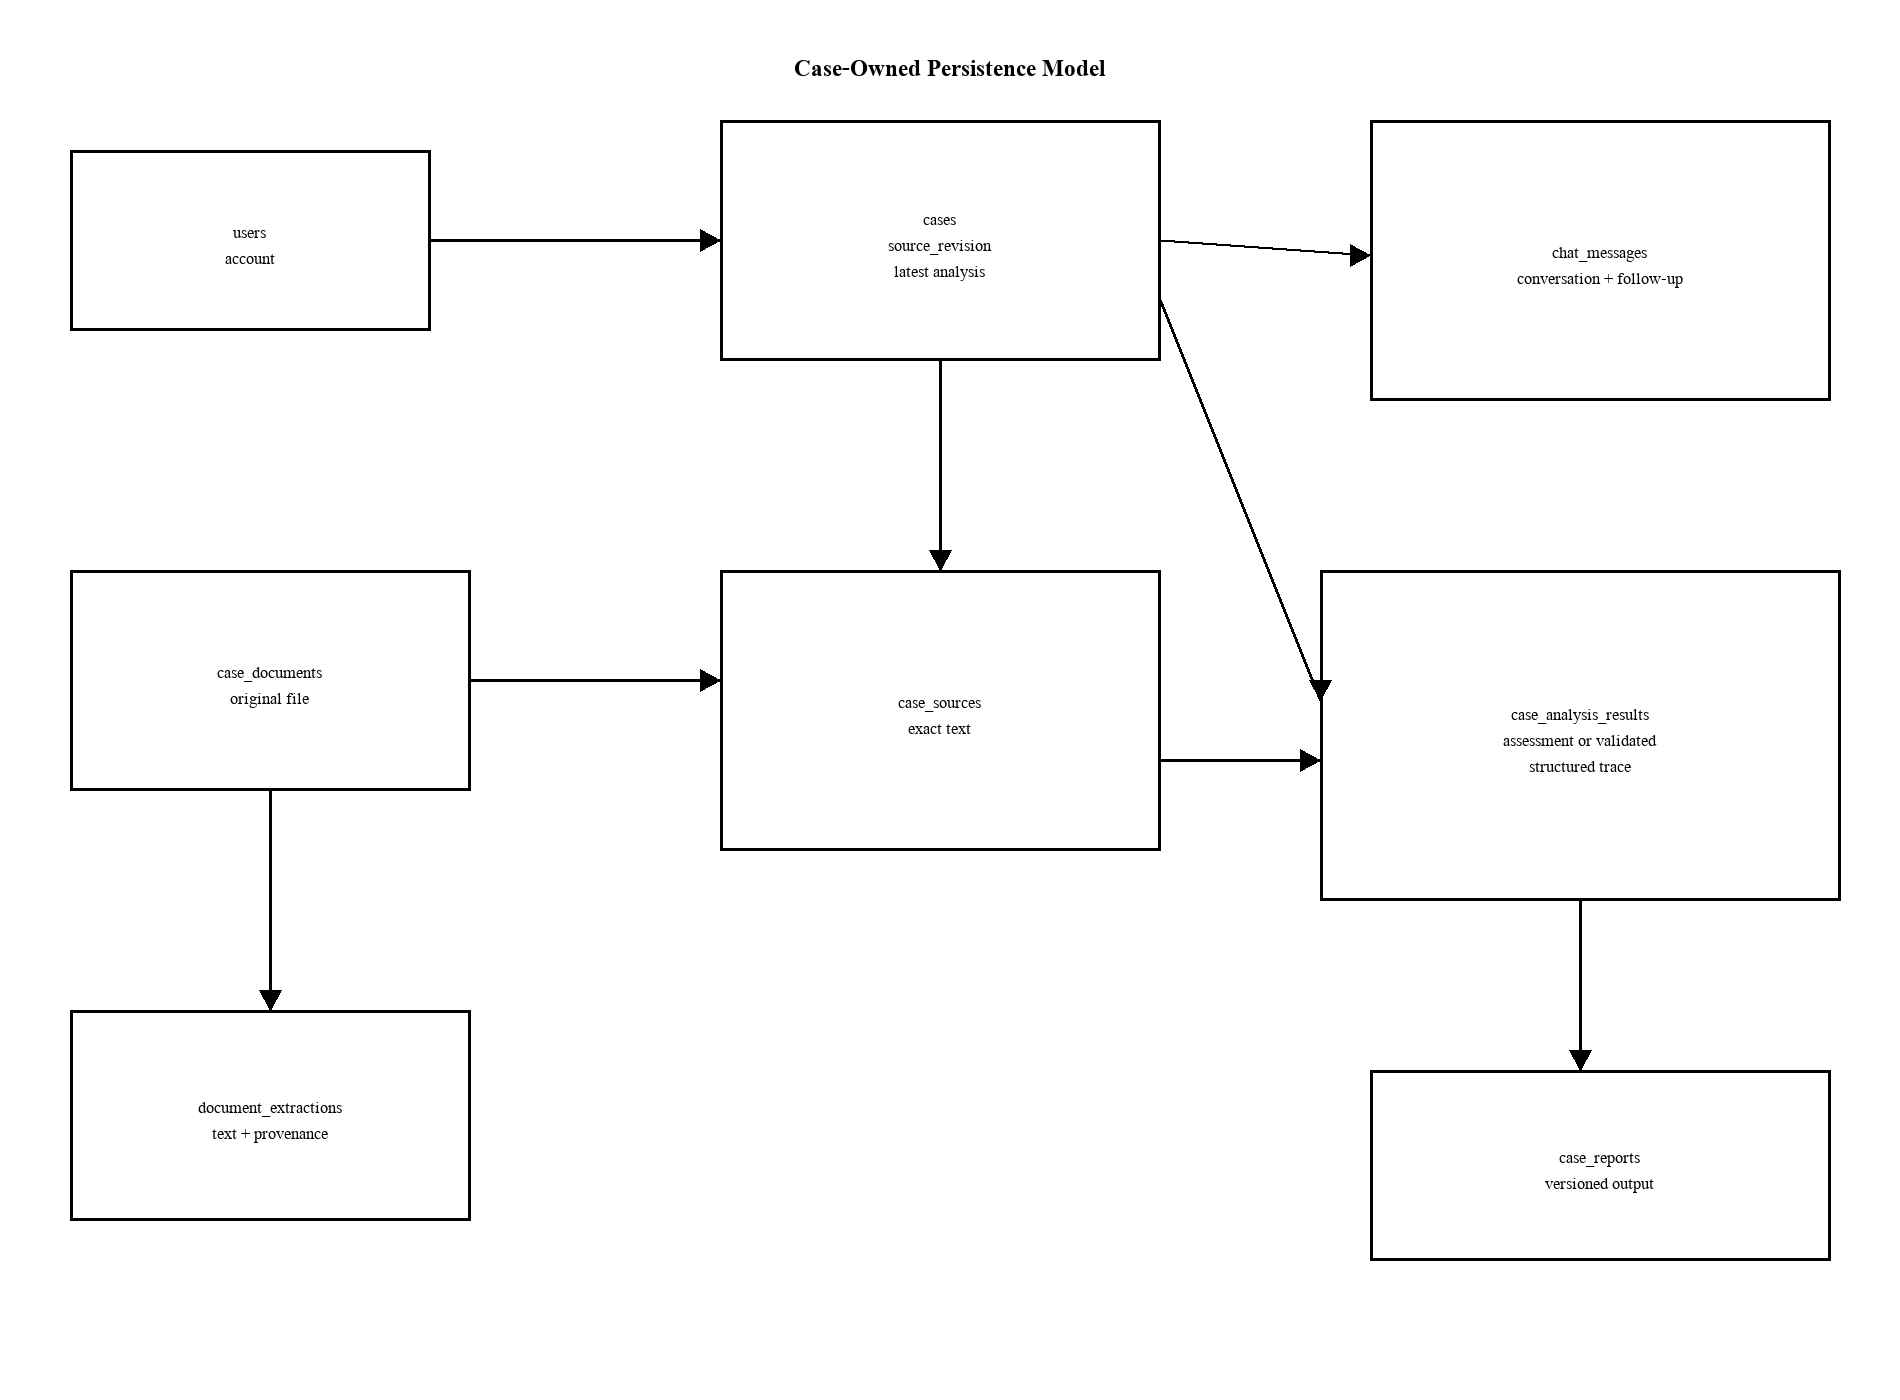
\includegraphics[width=0.96\textwidth]{figures/chapter4/figure-4-6.png}
\caption{Case-owned persistence model}\label{fig:4-6}
\end{figure}

\section{Report Generation}

A preliminary report is compiled from a stored validated analysis. The report service first selects the requested analysis result or the Case's latest result, then projects the trace, case sources, follow-up history, and technical augmentation into a fixed structured report contract. The report compiler is deterministic and does not make a new language-model call to rewrite the analysis.

The report contract contains seven fixed section identifiers: case summary, case evidence, MITRE ATT\&CK mapping, mapping rationale, evidence to examine, preliminary recommendations, and system limitations. Report claims retain support type, source identifiers, and optional MITRE technique identifiers. The assembly validator checks section count, claim identity, case-source membership, and technical-context membership before persistence.

One report is stored per analysis result. Requesting the same analysis again returns the existing report instead of creating a duplicate. New analysis results receive new case-level report versions. The stored report can be rendered as HTML for preview or as a PDF for download, while the report continues to identify the technical section as external context rather than incident evidence.

\begin{figure}[H]
\centering
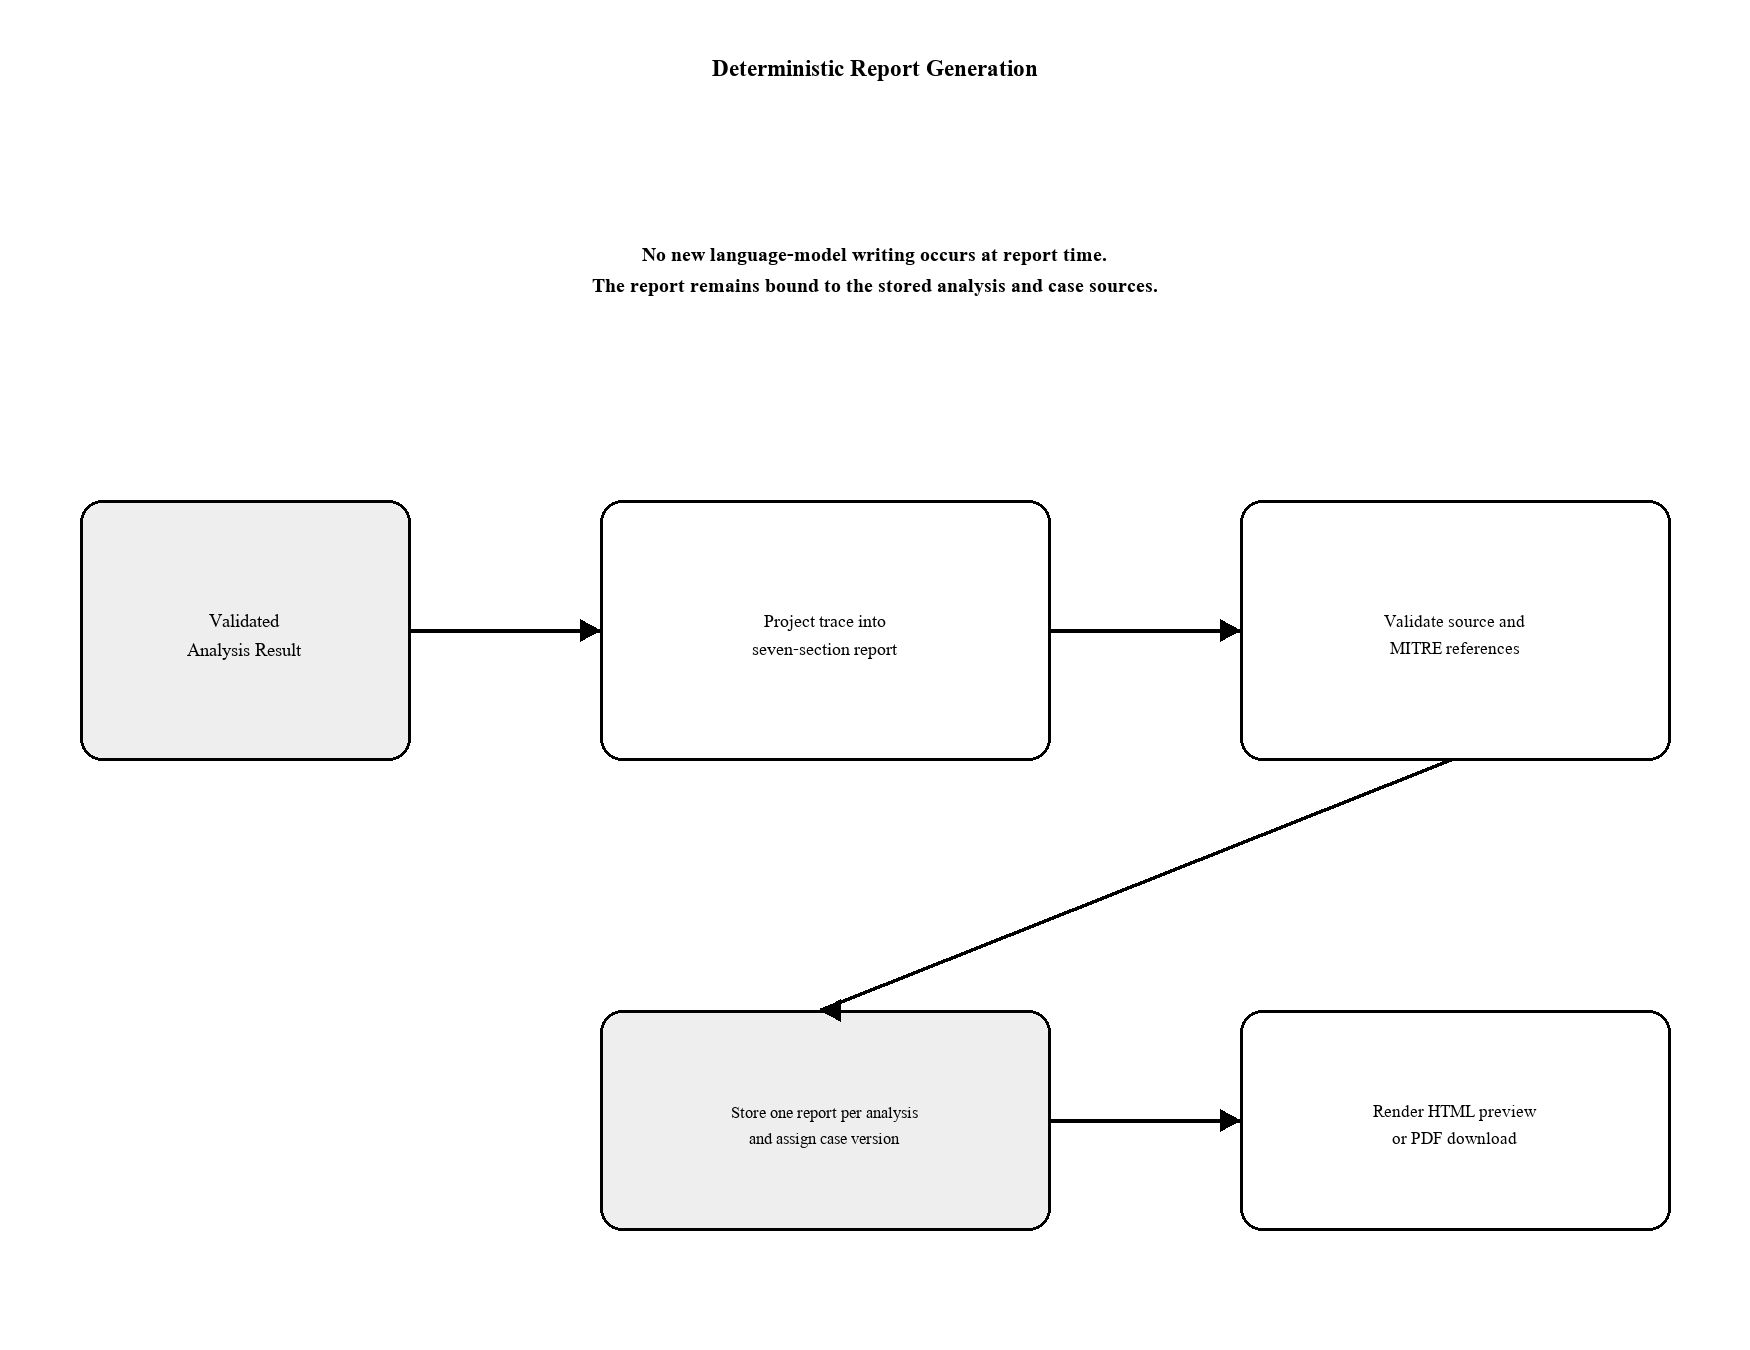
\includegraphics[width=0.96\textwidth]{figures/chapter4/figure-4-7.png}
\caption{Deterministic report generation and export}\label{fig:4-7}
\end{figure}

\section{Web Interface and Processing States}

The frontend is a Next.js App Router application organized around a case workspace. The case library opens a case, and the case layout owns the shared header and chat panel. The header exposes the active view, case title editing, analysis action, analysis-running state, and stale-result status. The Sources view handles narrative and document intake, while the Analysis view combines findings, technical context, source navigation, and report controls.

Server state is read through typed API functions and TanStack Query hooks. Queries cover the case, documents, sources, chat, analysis, and reports. Mutations update or invalidate only the related cache entries. The analysis mutation uses a case-specific mutation key so the workspace header can show one running state even when the user changes views during the request; this is a frontend state indicator and not a persisted run record.

The interface distinguishes a missing analysis, a current analysis, and a stale analysis by comparing the result source\_revision with the Case source\_revision. Finding cards expose source references and allow the reader to navigate to source material. Technical context has its own view and status presentation so that retrieved MITRE descriptions are visually and semantically separate from case findings.

The report component lists saved versions, requests generation only when a validated analysis exists, previews stored HTML, and downloads the selected PDF. These UI states follow the backend contracts rather than reconstructing workflow decisions in the browser.

\begin{longtable}{@{}>{\raggedright\arraybackslash}p{0.28\textwidth} >{\raggedright\arraybackslash}p{0.68\textwidth}@{}}
\caption{Case workspace views and data responsibilities}\label{tab:4-7}\\
\toprule
\textbf{View or component} & \textbf{Implementation responsibility} \\
\midrule
\endfirsthead
\textbf{View or component} & \textbf{Implementation responsibility} \\
\midrule
\endhead
Case library & Lists owned cases and opens a selected case workspace. \\
Sources view & Uploads documents, adds narrative text, shows extracted text, and exposes provenance. \\
Workspace header & Renames the case, selects the workspace view, starts analysis, and shows current or stale status. \\
Analysis view & Combines overview findings, conditional technical context, source navigation, and report controls. \\
Chat panel & Shows analysis-related conversation, receives general questions, and presents follow-up questions. \\
Report view & Generates one report per selected analysis, lists versions, previews HTML, and downloads PDF. \\
Query layer & Uses typed API functions and TanStack Query to share current case, source, chat, analysis, and report state. \\
\bottomrule
\end{longtable}

\begin{figure}[H]
\centering
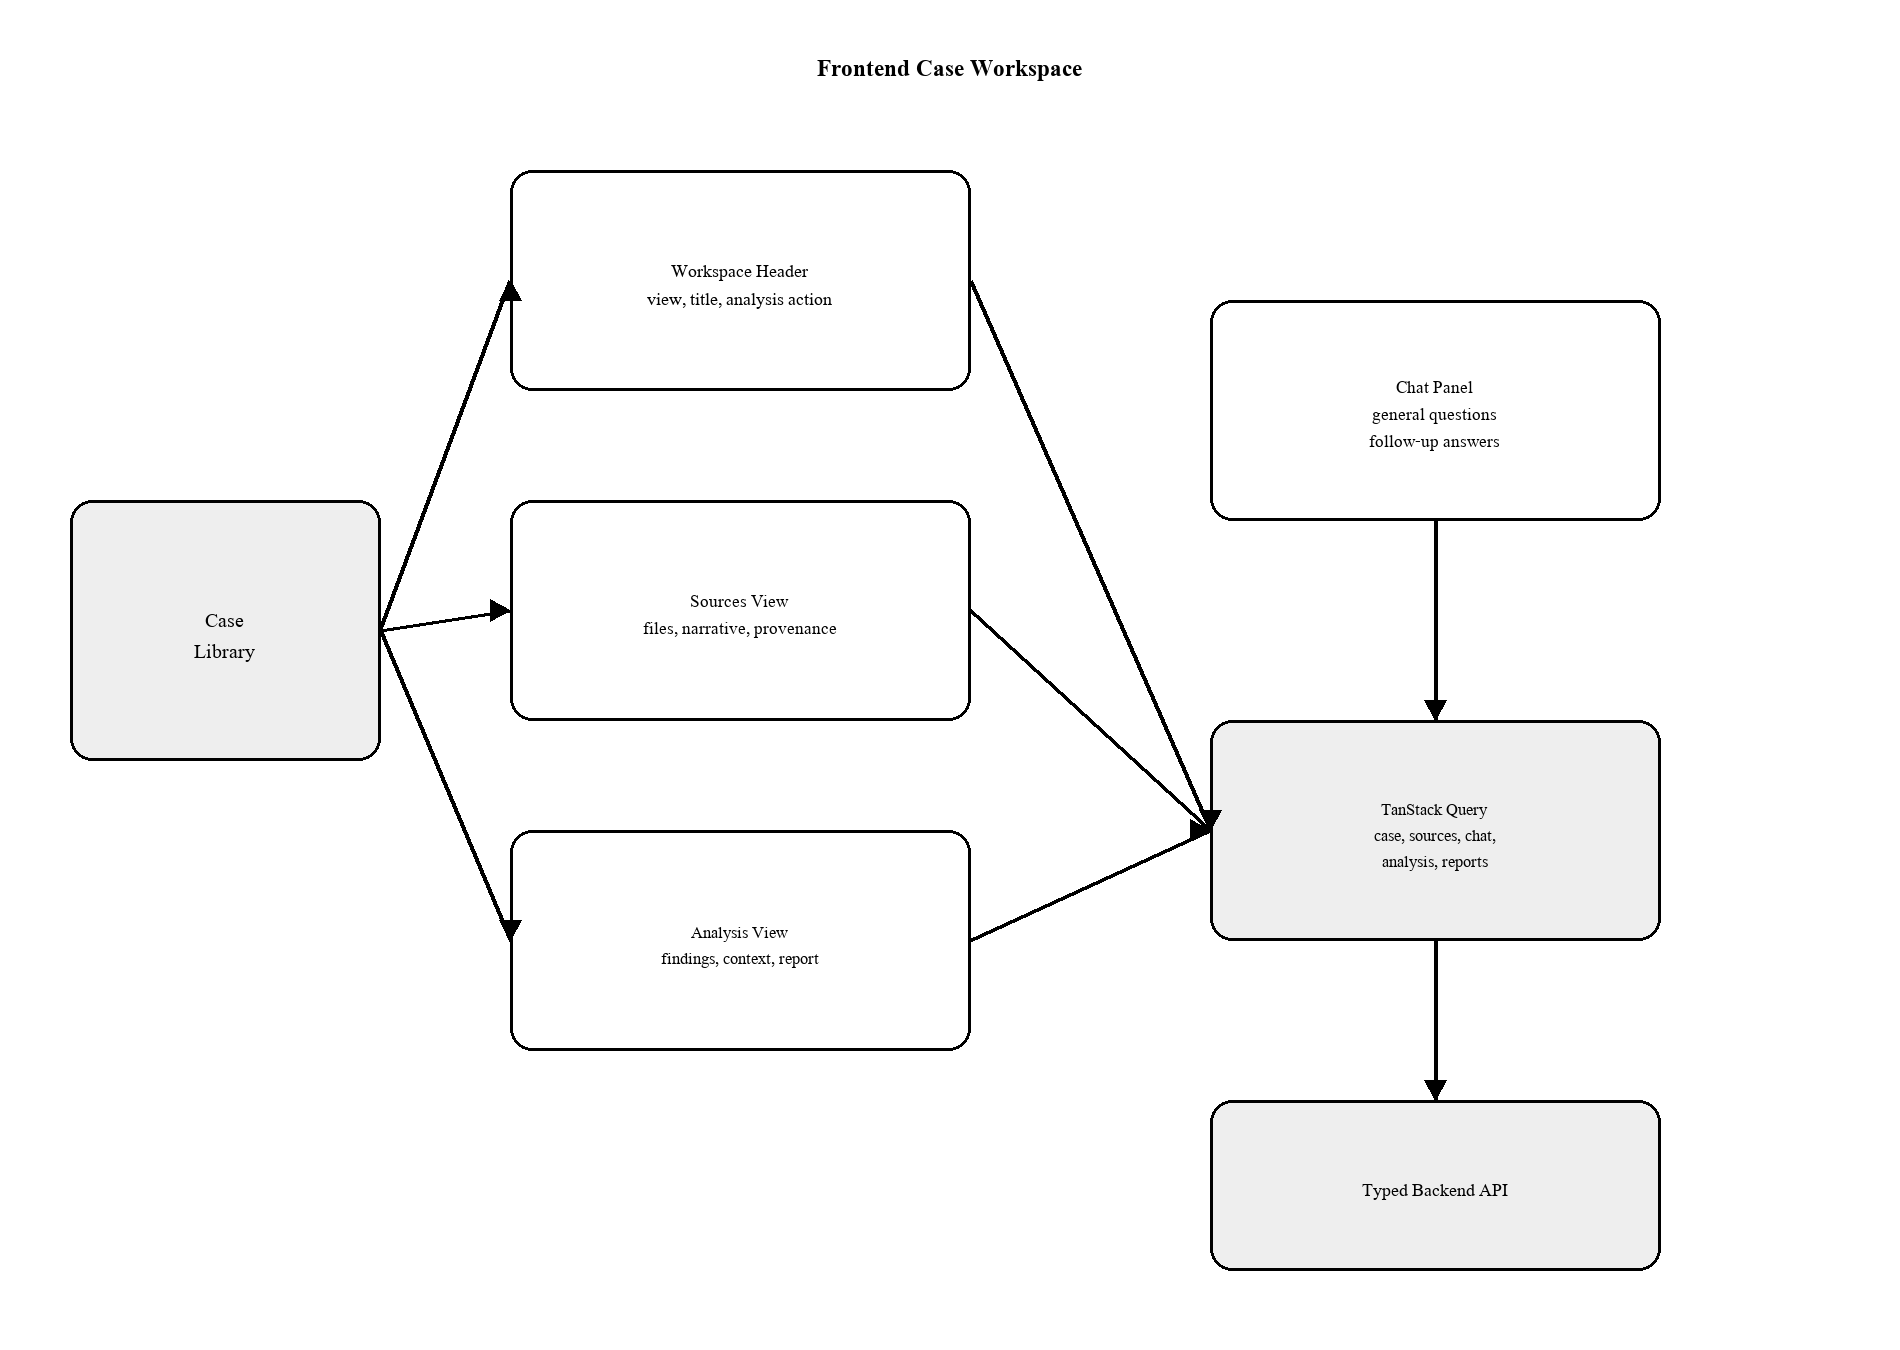
\includegraphics[width=0.96\textwidth]{figures/chapter4/figure-4-8.png}
\caption{Frontend case workspace and server-state flow}\label{fig:4-8}
\end{figure}

\section{Verification and Chapter Summary}

Verification is distributed across backend unit tests, PostgreSQL workflow tests, frontend component and hook tests, TypeScript checks, linting, and production-build checks. The repository tests the boundaries that can silently change the meaning of a case: route surface, source provenance, source-revision freshness, assessment short-circuiting, follow-up concurrency, technical-context isolation, structured report projection, and frontend cache updates.

The implementation does not claim that a valid quotation automatically proves that a claim is true. Binding verifies that a quotation can be located in a permitted source and records the limitation in the grounding report. Likewise, the presence of an ATT\&CK technique in the report means that external technical context was retrieved and accepted by the technical boundary; it does not prove that the technique occurred in the case.

In summary, CyberCase is implemented as a case-owned system with a traceable source-intake path, a request-scoped analysis workflow, deterministic follow-up policy, conditional technical augmentation, source-bound structured results, and deterministic report generation. The frontend presents these states through one case workspace while the Backend API remains the authority for ownership, validation, persistence, and stopping rules. These implementation properties provide the foundation for the experiments and system evaluation described in the following chapter.

\begin{longtable}{@{}>{\raggedright\arraybackslash}p{0.28\textwidth} >{\raggedright\arraybackslash}p{0.68\textwidth}@{}}
\caption{Verification coverage in the repository}\label{tab:4-8}\\
\toprule
\textbf{Area} & \textbf{Representative verification} \\
\midrule
\endfirsthead
\textbf{Area} & \textbf{Representative verification} \\
\midrule
\endhead
API surface & Route-surface checks assert the authenticated case routes and prevent unintended top-level resources. \\
Document intake & Parser, PDF fallback, Typhoon recognition, file limits, provenance, and warning behavior are tested. \\
Analysis & Assessment short-circuiting, structured contracts, source binding, freshness, MITRE augmentation, and failure states are tested. \\
Follow-up & Round limits, duplicate requests, concurrent answers, unanswered questions, and assessment persistence are tested. \\
Persistence & SQLAlchemy models are checked against Alembic schema expectations and PostgreSQL workflow tests. \\
Reports & Section structure, source and technique references, deterministic projection, HTML rendering, and PDF rendering are tested. \\
Frontend & Workspace components, hooks, chat, sources, technical context, reports, routes, TypeScript, lint, and production build are covered. \\
\bottomrule
\end{longtable}
